% !TEX encoding = UTF-8 Unicode
%Präambel

%Report für große Doukumente. Dieser ist in Kapitel (\chapter{}) aufgeteilt
%\documentclass[12pt, a4paper, ngerman]{report} 

%Article für normale Doumente
\documentclass[12pt, a4paper, ngerman]{article}

%Deutsche Beschreibungen von generiertem Text (table of contents => Inhaltsverzeichnis)
\usepackage[ngerman]{babel}

%Umlaute
\usepackage[utf8]{inputenc}

%Schriftart Helvetica 
\usepackage[scaled]{helvet}

%Seitenränder
\usepackage{geometry}
%top = Abstand nach oben
%left = Abstand nach links
%right = Abstand nach rechts
%bottom= Abstand nach unten
%heapsep= Abstand zwische Kopfzeile und Text
%footskip= Abstand zwischen Text und Fußzeile
\geometry{a4paper, top=25mm, left=30mm, right=25mm, bottom=30mm, headsep=10mm, footskip=12mm}

%Farben nutzen
\usepackage{xcolor}

%Grafiken einbinden
\usepackage{graphicx}

%Zusätzliche Positionsbefehle
\usepackage{float} 

%Die Einrücktiefe bei einem neuen Absatz
\setlength{\parindent}{0pt}


%Fülltext
\usepackage{blindtext}

%Fuer Zitate	
\PassOptionsToPackage{backend=bibtex}{biblatex}
\usepackage[natbib=true,style=numeric]{biblatex}
\usepackage[babel,german=guillemets]{csquotes}
\bibliography{quellen.bib} 


%Eigene Kommandos
% Osi Modell
\newcommand{\osi}{ISO/OSI Referenzmodell\xspace}

%Ende Präambel
	
\begin{document}

\begin{titlepage}
		\begin{center}
			
\includegraphics[width=.8\linewidth]{Grafiken/logo_htw.jpg}\\[1cm]    
			\textsc{\LARGE Hochschule für Technik und Wirtschaft \newline Fakultät für Ingenieurwissenschaften}\\[1.5cm]
			\newcommand{\HRule}{\rule{\linewidth}{0.5mm}} \HRule \\[0.4cm] { \huge \bfseries Ausarbeitung Protokolle}\\[0.4cm]
			\HRule \\[1.5cm]

			\begin{minipage}{0.4\textwidth}
				\begin{flushleft} \large
					\emph{Autoren:}\\
					Deniz Kadiogullatri 3553892\\
					Christoph Drost 3576450
				\end{flushleft}
			\end{minipage}
			\hfill
			\begin{minipage}{0.4\textwidth}
				\begin{flushright} \large
					\emph{Betreuer:} \\
					Jonas Vogt, M.Sc.
				\end{flushright}
			\end{minipage}
			\vfill
			{\large \today}
		\end{center}
	\end{titlepage}


%Inhaltsverzeichnis auf eigener Seite
\tableofcontents
\newpage 

\section{Einleitung}
Im Folgenden sollen verschiedene Layer 2 Protokolle für kabelgebundene Netze miteinander verglichen werden. Um die Zusammenhänge besser erklären zu können, möchten wir erst auf das \osi eingehen.
\subsection{Das \osi}
\begin{figure}[h]
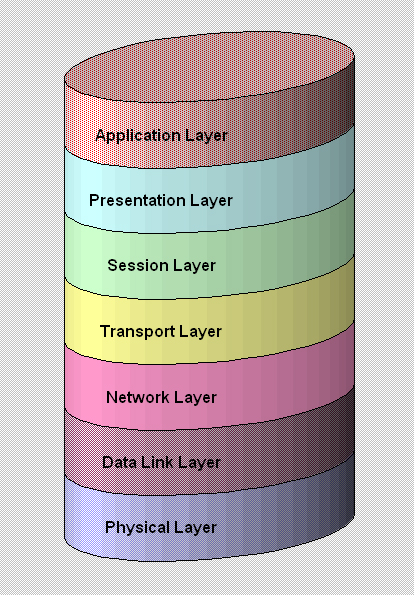
\includegraphics[width=0.5\textwidth]{Grafiken/osi_modell.jpg}
\caption{Das \osi im Überblick \cite{osi_modell}}
\label{osi_modell}
\end{figure} 
Diese Grafik stellt die Schichten des \osi da. Das \osi, (Open Systems Interconnection Model) ist ein allgemeines Kommunikationsmodell,  das die Kommunikation unterschiedlichster Geräte ermöglicht. Es beschreibt ein komplettes Telekommunikationsnetzwerk. Die einzelnen Funktionen sind in 7 Schichten aufgeteilt. 

Das \osi standardisiert die Netzwerk Architektur. Dadurch können Hersteller Lösungen anbieten, die auf der ganzen Welt genutzt werden können. Eine proprietäre Lösung hätte zu Insellösungen geführt. Ein weiterer Vorteil ist, dass die einzelnen Schichten, oder Layer, über Schnittstellen miteinander kommunizieren. Das ermöglicht ein Austauschen einzelner Komponenten, ohne die gesamte Architektur ändern zu müssen.

Da das \osi nur ein Referenzmodell darstellt, müssen die einzelnen Schichten konkret implementiert werden. Diese Implementierungen sind eigene Protokolle. 

\subsection{Der Layer 2}
Der Layer 2, Data Link Layer, setzt auf dem Physical Layer auf und stellt dem Network Layer seine Dienste zur Verfügung. Der Physical Layer beschriebt das Medium über das die Signale übertragen werden. Hier findet noch keine Logik statt. 

Die Aufgaben des Layer 2 im Überblick:
\begin{itemize}
	\item Aufteilung in Pakete
	\item Fehlerkontrolle
\end{itemize} 

\subsubsection{Aufteilung in Frames}
Die Datenblöcke werden im Layer 2 in Frames aufgeteilt. Die Vorteile des Framing sind die schnellere Nutzung eines shared Mediums und dass fehlerhafte Daten nicht komplett übertragen werden müssen.
\subsubsection{Fehlerkontrolle}
Der Data Link Layer führt eine Fehlerkontrolle durch. Dazu zählen eine Suche nach Duplikaten, nach inkorrekt oder unvollständig gesendeten Paketen. Wenn ein Fehler entdeckt wird, wird eine neue Übertragung der Frames angefordert \cite[S. 91]{SWB-107223570}. Die Fehlerkontrolle wird über den \glqq Cyclic Redundancy Check\grqq ~CRC durchgeführt. Dieses Verfahren ist eine Möglichkeit zur Prüfsummenberechnung, die beim Sender und der Senke durchgeführt wird. Sind beide Prüfsummen gleich, kann angenommen werden, dass das Frame korrekt übertragen wurde. 

Die Frames werden mit Sequence Numbers durchnummeriert. Der Empfänger prüft, ob die Frames in der richtigen Reihenfolge ankommen. Bei einer \glqq out-of-sequence transmission\grqq ~kann von einem verlorenen Frame ausgegangen werden, das entsprechende Frame wird neu angefordert, bzw. Layer 3 wird benachrichtigt.
\section{Die Layer 2 Protokolle im Überblick}

\subsection{Ethernet}
Ethernet ist ein weit verbreitetes Layer 2 Protokoll. 90\% aller lokal installierten Netzwerke sind mit Ethernet realisiert\cite{SWB-097965316}. Ethernet wurde ursprünglich für die Anbindung eines Druckers bei der Firma Xerox Corporation entwickelt. Die damalige Übertragungsgeschwindigkeit von 2,94 Mbit/s wurde auf aktuell 100 Gbit/s gesteigert, weitere Steigerungen sind zu erwarten.

Die Daten werden im Ethernet über einen eigenen Übertragungskanal transportiert. Kollisionen werden durch \glqq CSMA/CD\grqq ~entdeckt, bzw. aufgelöst. Die Übertragung läuft gleichberechtigt und verbindungslos. Die Daten werden an alle Teilnehmer weitergeleitet, diese vergleichen die Empfängeradresse mit ihrer eigenen und verwerfen die Frames, die nicht an sie adressiert sind. Diese Aussage kann eingeschränkt werden, da Switche die Daten nur an Ports leiten, an denen die entsprechenden Senken angeschlossen sind. 

\subsubsection{Gebräuchliche Übertragungsmedien des Ethernet}
\begin{figure}[H]
\begin{minipage}[hbt]{.28\linewidth}
	\centering
	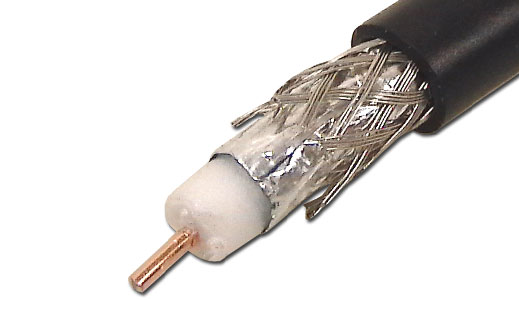
\includegraphics[width=0.9\linewidth]{Grafiken/koaxkabel.png}
	\caption{Koaxkabel \cite{koax_kabel}}
	\label{koaxkabel}
\end{minipage}
\hfill
\begin{minipage}[hbt]{.28\linewidth}
	\centering
	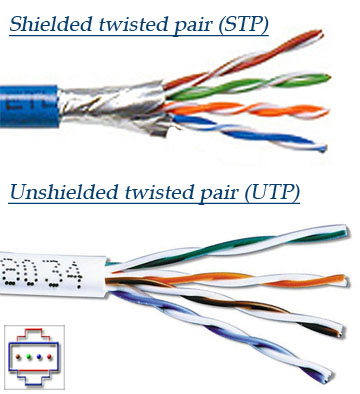
\includegraphics[width=0.9\linewidth]{Grafiken/twistetPair.jpg}
	\caption{Twistet Pair Kabel \cite{tw_kabel}}
	\label{twkabel}
\end{minipage}
\hfill
\begin{minipage}[hbt]{.28\linewidth}
	\centering
	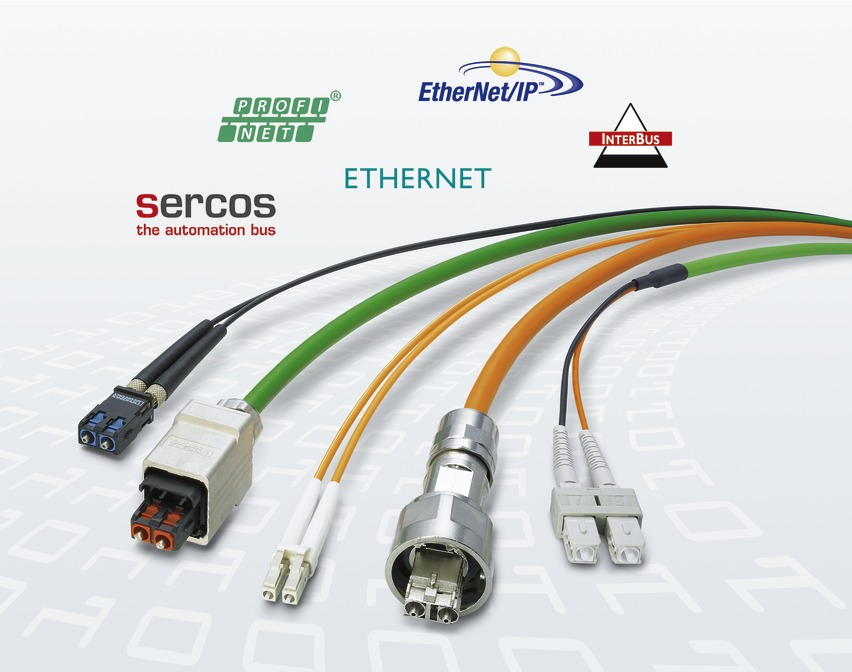
\includegraphics[width=0.9\linewidth]{Grafiken/lwl_leiter.jpg}
	\caption{Lichtwellenleiter \cite{lwl_leiter}}
	\label{lwlleiter}
\end{minipage}
\end{figure}
 
Historisch gesehen muss das Koaxialkabel als Medium des Ethernet genannt werden. Das Koaxkabel wurde 1990 mit der Einführung von 10BaseT (IEEE 802.3i) durch Unshielded Twisted Pair Kabel ersetzt. Ab 1998 wurden mit der Einführung des Gigabit Ethernet auch Lichtwellenleiter genutzt. 

\subsubsection{Zugriff auf das Medium}
Historisch gesehen nutzt Ethernet das Übertragungsmedium als Shared Medium. Die einzelnen Teilnehmer wurden am selben Koaxialkabel über T-Stücke angeschlossen. Um Kollisionen zu vermeiden, wurde ein geeignetes Verfahren zur Vermeidung benötigt. Von einer Kollision spricht man, wenn mehrere Teilnehmer gleichzeitig auf das Medium zugreifen würden, also Signale aussenden. Die Signale würden sich gegenseitig überlagern und wären nicht mehr nutzbar. Bei Ethernet wird CSMA/CD eingesetzt. Bei diesem Verfahren wird vor dem Senden geprüft, ob die Leitung frei ist. Erst wenn die Leitung frei ist wird gesendet (Carrier Sense). Wenn zufällig mehrere Teilnehmer gleichzeitig ein Signal aussenden (Multiple Access) kommt es dennoch zu Kollisionen. Der/Die Sender prüfen während dem Senden, ob es zu Kollisionen kommt (Collision Detect) und brechen ihre Übertragung im Fall einer Kollision ab. Nach einem Abbruch wird eine zufällige Zeit gewartet bis erneut gesendet wird. Der Grund, warum es trotz diesem Verfahren zu Kollisionen kommen kann, ist die Signallaufzeit. Die Signale brauchen eine gewisse Zeit um über die Leitungen übertragen zu werden. 

In seinen Anfangszeiten übertrug Ethernet im Halbduplex Verfahren. Das bedeutet, dass ein Übertragungskanal zum Senden und zum Empfangen genutzt wird. Dadurch halbiert sich natürlich im schlimmsten Fall die Datenrate. Mit der Einführung von Twisted Pair Kabeln und Lichwellenleitern wurde Ethernet auf den Vollduplex Betrieb umgestellt. Dadurch konnte die Übertragungsrate gesteigert werden und Kollisionen wurden unwahrscheinlicher.
\begin{figure}[H]
	\centering
	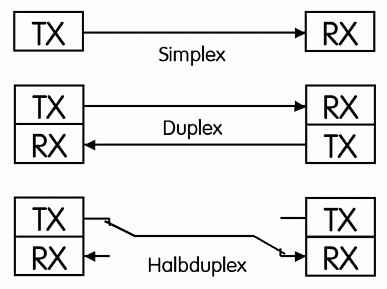
\includegraphics[width=0.4\linewidth]{Grafiken/duplex.jpg}
	\caption{Unterschied der Duplex Übertragungen \cite{duplex}}
	\label{duplex}
\end{figure}
 
 \subsubsection{Frames}
Um Daten über Ethernet übertragen zu können werden sie in Frames aufgeteilt. Der Vorteil daran ist, dass ein Sender bei großen Übertragungen nicht das gesamte Netzwerk belegt und dass bei einer fehlerhaften Übertragung nur einzelne Frames neu versandt werden müssen. Der Ausdruck Frame kann wörtlich genommen werden. Die Nutzdaten werden in einen Rahmen (Frame) eingepackt.

Neben den eigentlichen Nutzdaten enthält ein Frame:
\begin{itemize}
	\item Die Präambel (dient u.a. zur Synchronisation der Empfängerstationen) 
	\item Die Hardware Quell- und Zieladresse
	\item Ein Typ- oder Längenfeld
	\item Eine Checksumme
\end{itemize}
\begin{figure}[H]
	\centering
	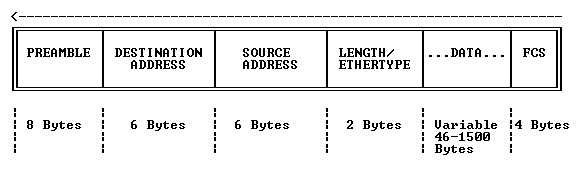
\includegraphics[width=0.9\linewidth]{Grafiken/ethernet_frame.jpg}
	\caption{Ethernet 802.3 Frame \cite{ethernet_frame}}
	\label{ethernet_frame}
\end{figure}

Die Präambel enthält eine Bitfolge, die dem Empfänger signalisiert, dass ein Rahmen ankommt. Die Präambel besteht aus 8 Bytes mit einer alternierenden Folge aus 0 und 1. Die letzten 2 Bits im letzten Byte sind immer 1. Hier besteht ein kleiner Unterschied zwischen DIX und IEEE. Obwohl die Bitfolgen die gleichen sind, ist die Präambel im IEEE Standard formell in die 7 Byte lange Präambel und den 1 Byte langen Start-of-Frame-Delimiter aufgeteilt.
 
Die Adressen sind MAC Adressen. Dieser werden von der IEEE an die Hersteller von Ethernet Komponenten vergeben und müssen weltweit eindeutig sein.

\subsubsection{Topologie}
Ethernet ist keiner bestimmten Netzwerk Topologie zuzuordnen. Heute gebräuchlich ist eine Sterntopologie, andere Formen sind aber auch möglich.   


\subsection{LAPD}
\blindtext

\subsection{PPP}
Router - Router und Host - Netzwork Verbindungen über synchrone und asynchrone Kreise. Enthält ein Protokoll Feld um das Network Layer Protokoll zu Identifizieren \cite[S. 102]{SWB-107223570}  

Während in einzelnen Gebäuden meist LANS zum Einsatz kommen, werden für die weitreichende Verbindungen meist Punkt-zu-Punkt-Standleitungen eingesetzt. Diese Leitungen verbinden weit entfernte Router miteinander, hinter denen LANS mit mehren Hosts wie Personal-Computer, Workstation oder Server angeschlossen sein können. Die Verbindung in die Außenwelt von diesen LANS aus, wird eben genau über diese Router laufen. Und hier kommt das PPP (Point-to-Point Protocol) zum Einsatz.

PPP ist in RFC 1661 definiert und wurde in mehreren anderen RFCs weiter ausgearbeitet wie in RFC 1662 und 1663.

Das Protokoll unterstützt Fehlererkennung, dynamische IP-Adressen Vergebung bei Verbindungsaufbau, Berechtigungsprüfung und mehrere Protokolle.

Das PPP umfasst desweiteren noch ein ganzes weiteres Protokoll das zum Aktivieren und Testen einer Leitung als auch zum Verhandeln von verschiedenen Parametern die für das PPP wichtig sind und zum Beenden nicht mehr gebrauchten Verbindungen verwendet wird. Die Aushandlung findet über ein eigenes Protokoll das sogenannte Link Control Protocol, im folgenden kurz als LCP bezeichnet, statt. LCP wird innerhalb des PPP Frames als Nutzdaten übertragen.

Ausserdem ermöglicht PPP es der Vermittlungsschicht (Networklayer) das für auf dieser Schicht laufende Protokoll, von diesem Protokoll unabhängige Optionen auszuhandeln, diese nennt man Network Control Protocol (NCP), so das auf jeder unterstützten Vermittlungsschicht ein anderes NCP laufen kann. 

Beispiele für NCP sind IPCP, AppleTalk Control Protokoll oder IPXCP. Das IPCP steht für IP Control Protocol und wird zur unter anderem zur IP-Vergabe genutzt.


\subsection{LCP Verhandlung}


Das Verbindungssteuerungs-Protokoll (Link-Control Protolcol - LCP) des PPP stellt eine Methode für die Etablierung, Konfigurierung, Verwaltung und Beendigung einer Punkt-zu-Punkt-Verbindung zur Verfügung. LCP durchläuft vier einzelne Phasen:
In der ersten Phase erfolgt der Verbindungsaufbau, und die Konfiguration wird ausgehandelt. Bevor irgendwelche Datagramme der Vermittlungsschicht (z.B. IP) ausgetauscht werden können, muß LCP die Verbindung erüffnet und Konfigurationsparameter ausgehandelt haben. Diese Phase ist beendet, wenn sowohl ein Frame gesendet als auch einer empfangen wurde, der die Konfigurationsbestöätigung enthält.
Dann wird die Verbindungsqualität ermittelt. Diese Phase ist optional. In dieser Phase wird die Verbindung getestet, um festzustellen, ob die Qualität dafür ausreicht, daß die Protokolle der Vermittlungsschicht gestartet werden können. LCP kann die Übertragung von Protokoll-Informationen der Vermittlungsschicht so lange hinauszögern. bis diese Phase beendet ist.
Zu diesem Zeitpunkt erfolgt die Konfigurationaushandlung des Vermittlungsschicht-Protokolls. Nachdem LCP die Phase der Qualitätsprüfung beendet hat, können die Vermittlungsschicht-Protokolle vom entsprechenden NCP einzeln konfiguriert werden und jederzeit gestartet oder beendet werden. Wenn LCP die Verbindung beendet, informiert es die Protokolle der Vermittlungsschicht, damit diese entsprechende Schritte einleiten.
Zuletzt erfolgt die Verbindungsbeendigung. LCP kann die Verbindung jederzeit beenden. Eine Verbindung wird im allgemeinen auf Anforderungen eines Benutzers beendet, kann aber auch aufgrund eines physischen Ereignisses beendet werden, z.B. wenn das Trägersignal verloren geht oder ein Timer abläuft.
Es gibt drei Klassen von LCP-Frames. Verbindungsaufbau-Frames dienen dazu, eine Verbindung aufzubauen und zu konfigurieren. Verbindungsbeendigungs-Frames dienen dazu, eine Verbindung zu beenden, während Verbindungsverwaltungs-Frames eine Verbindung verwalten und debuggen.

Diese Frames werden für die Durchführung der einzelnen LCP-Phasen benötigt.

Das LCP befasst sich nicht mit den Optionen selbst die für Schicht-2 ausgehandelt werden sondern nur wie sie ausgehandelt werden. Ein Prozess kann seine Optionen einem anderen vorschlagen und dieser kann dann entscheiden ob er alle annimmt oder nur einige annimmt oder sie ganz abschlägt. Es gibt in RFC 1661 elf verschiedene Typen von LCP-Rahmen die diese verhalten festhalten. 

Im folgenden die einzelnen Typen und ihre Bedeutung:

\begin{itemize}
	\item Configure-request	- Liste der vorgeschlagenen Optionen und Werte
	\item Configure-ack		- Alle Optionen werden angenommen
	\item	Configure-nak		- Einige Optionen werden nicht angenommen
	\item Configure-reject	- Einige Optionen können nicht Verhandelt werden
	\item Terminate-request	- Anforderungen zum Trennen der Verbindung
	\item Terminate-ack		- Verbindung wurde getrennt
	\item Code-reject		- Unbekannte Anforderungen erhalten
	\item Protocol-reject		- Unbekanntes Protocol angefordert
	\item Echo-request		- Anforderungen, den Rahmen zurückzusenden
	\item Echo-reply		- Rückgabe des Rahmens
	\item	Discard-request	- Rahmen verwerfen (für Testzwecke)
\end{itemize} 



\subsection{Verbindungsablauf des PPP}

Im folgenden durchlaufen wir die verschiedenen Zustände des Verbindungsaufbaus bis hin zum Abbau der Verbindung anhand der unten gezeigten Zeichnung.
Als ersten ist die Leitung tot. Das bedeutet es existiert kein Träger auf der physikalischen Ebene und auch keine Verbindung auf der Bitübertragungsschicht.
Nachdem eine physikalische Verbindung aufgebaut worden ist wechselt der Zustand zu Aufbauen. Genau in diesem Augenblick beginnt dann die Verhandlung der LCP Optionen. Wenn diese erfolgreich sein sollten können nun die beiden Parteien die mit einander kommunizieren möchten ihre Identität prüfen. Das heisst der Zustand wechselt auf Authentifizieren. Falls dieser Fall nun fehlschlägt wird die Verbindung Beendet, dh. auch der Zustand ändert sich und der Träger wird wieder freigegeben. Somit wären wir wieder im Ausgangszustand. Im Gegengesetzten Fall würde der nächste Zustand Netz heissen und das entsprechende NCP-Protokolle aufgerufen werden um die Vermittlungsschicht zu konfigurieren. Nach dem die Konfiguration erfolgreich abgeschlossen ist wechselt der Zustand nach Öffnen in der die eigentliche Datenübertragung stattfindet. Wenn diese Beendet ist und alle Daten erfolgreich übertragen worden sind kann die Verbindung wie bereits oben geschrieben Beendet werden.

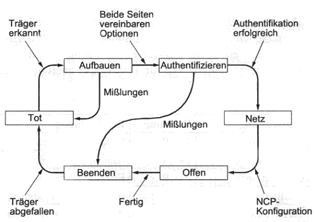
\includegraphics[width=1\textwidth]{Grafiken/ppp.jpg}


\subsubsection{Frames}

Das PPP besitzt eine Rahmenbildungsmethode die Anfang und Ende eines jeden Rahmens kennzeichnet. Diese übernimmt ebenfalls die Aufgabe der Fehlererkennung

Der Rahmen besteht aus insgesamt sieben Feldern. Dazu gehören Flag, Adress, Steuerung,  Protokoll, Nutzdaten, Prüfsumme und wieder Flag.

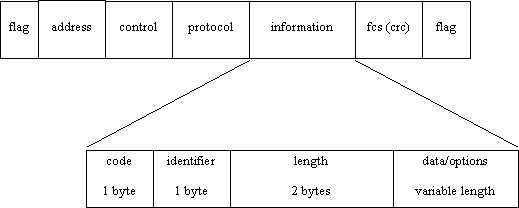
\includegraphics[width=1\textwidth]{Grafiken/ppp-frame.jpg}

\subsubsection{Flag}

Das Flag besteht am Anfang wie am Ende aus einem Byte (011111110) dieses wird mit der Byte-Stuffing-Methode aufgefüllt, um zu verhindern das im Datenfeld eines Frames eine Bitfolge als Sternzeichen interpretiert werden. Das erste Byte ist somit das Startbyte für einen Rahmen. Am Ende eines Rahmens wird die selbe Bitfolge gesendet und zu kennzeichnen das der Frame zu Ende ist.


\subsubsection{Adress}

Das Adressfeld steht immer auf einem festen Wert und zwar aus acht mal eins. Dies dient dazu das alle Stationen den Rahmen akzeptieren und zum vermeiden das Verbindungsadressen zugewiesen werden müssen. Da dieses Feld in der Standartkonfiguration immer gleich ist, gibt es wie auch bei dem Steuerungsfeld einen die Möglichkeit zwischen zwei Parteien diese Felder einfach entfallen zu lassen und damit zwei Byte pro Rahmen einzusparen.


\subsubsection{Steuerung}

Das Feld Steuerung, als Standardwert 00000011, zeigt einen unnumerierten Rahmen an. PPP bietet keine zuverlässige Übertragung mit Folgenummern und Bestätigungen. Es ist allerdings möglich eine solche Übertragung zu realisieren. Die genauen Details sind in RFC 1663 definiert, die jedoch in der Praxis nicht häufig eingesetzt werden.


\subsubsection{Protokoll}

Das vierte Feld, Protokoll, gibt an welche Art von Paket in den Nutzdaten übertragen wird. Dies können beispielsweise LCP, NCP, IP, IPX und andere Protokolle sein. Normalerweise ist die Größe des Feldes auf zwei Byte festgelegt, es ist jedoch möglich über das LCP auf ein Byte runter zu handeln.


\subsubsection{Nutzdaten}

Die große des Feldes Nutzdaten wird üblicherweise von den Parteien ausgehandelt und festgelegt. Findet dieser Prozess über das LCP nicht statt so ist das Feld standardmäßig auf 1.500 Byte festgelegt.
Wenn es nicht genug Daten geben sollte um ein Frame zu füllen kann über Padding dieses auch bei Bedarf aufgefüllt werden.

\subsubsection{Prüfsumme}

Die Prüfsumme kann auf bis 4 Byte ausgehandelt werden, im Normalfall reichen aber 2 Byte aus. Sie dient zum überprüfen ob der Rahmen richtig gesendet worden ist.


\section{Bedeutungen der Protokolle im \osi }

%indirekte Quellen einbinden
\nocite{*} 

%Quellenangabe auf eigener Seite
\newpage
\sloppy
\printbibliography 



%Abbildungsverzeichnis auf eigener Seite
\newpage
\listoffigures

\end{document}